\documentclass[aspectratio=169]{beamer}

\usepackage[utf8]{inputenc}

\usepackage{amsfonts}
\usepackage{amsmath}
\usepackage{color}
\usepackage{listings}
\usepackage{tikz}
\usepackage{hyperref}

\newif\ifnotes
  \notesfalse
%  \notestrue

\newif\iftransitions
% \transitionstrue
 \transitionsfalse

\newif\iffast
% \fasttrue
  \fastfalse

\ifnotes
\usepackage{pgfpages}
\setbeameroption{show notes}
\setbeameroption{show notes on second screen=right}
\fi

\usetheme{Rochester}
\usecolortheme{beaver}

\addtobeamertemplate{navigation symbols}{}{%
    \usebeamerfont{footline}%
    \usebeamercolor[fg]{footline}%
    \hspace{1em}%
    \insertframenumber/\inserttotalframenumber
}

\lstloadlanguages{C++}
    \lstset{%
        language={C++},
        basicstyle=\ttfamily,
        keywordstyle=\color{blue},
        showstringspaces=false,
        escapechar={§},
        escapeinside={(*@}{@*)}
    }

\lstdefinestyle{cpp20}{language={C++},
  morekeywords={noexcept,co_await,co_return,co_yield,requires,consteval,constinit,concept}
}

\tikzstyle{every picture}+=[remember picture]

\newcommand{\cpause}{\iftransitions \pause \fi}

\newcommand{\cuncover}[2]{\iftransitions \uncover<#1>{#2} \else #2 \fi}

\definecolor{co_return_object}{RGB}{179,179,255}
\definecolor{co_promise}{RGB}{255,179,179}
\definecolor{co_awaitable}{RGB}{179,255,179}


\title{Building Interfaces That Are Hard to Use Incorrectly}
\author{Andreas Weis}
\institute{Woven by Toyota}

\date{C++ On Sea 2023}
\titlegraphic{
\includegraphics[height=.15\textheight]{resources/cpponsea-logo.png}}

\iffalse
Building Interfaces That Are Hard to Use Incorrectly

C++ is a language with many sharp edges. Besides the core language providing plenty of features that allow users to shoot themselves in the foot, higher-level library interfaces are also often designed with complex preconditions, the violation of which can again lead to undefined behavior and results that are just as unpredictable as what results from misuse of a lower level language feature. Fortunately, through clever use of the C++ type system we can design interfaces in a way that makes them much harder to misuse accidentally and drastically reduce the opportunities for bugs in user code.

In this talk, we will present a number of design techniques that allow library designers to reduce the possibilities of misuse by their users, by pushing the detection of precondition violations from run-time to compile-time.  We will show how to distinguish different categories of preconditions and how we can use the C++ type system to prevent accidental violation of those preconditions at run-time. We will demonstrate with a number of code samples how the use of such type-based techniques prevents interface misuse in practice and take a look at the trade-offs that arise from such an approach.

Brief
A collection of design techniques for hardening library interfaces against misuse and catching common user errors at compile time.

Outline:
- Interface Design Guidelines - "Make Interfaces Easy to Use Correctly and Hard to Use Incorrectly"
- Examples for interfaces that are easy to use incorrectly in popular libraries
- A categorization of precondition violations
- Minimizing the possibility for precondition violations through the type system
-- Restricting access to data (encapsulation techniques; opaque types; enforcing structured data access for flexible data layouts; limited friendship)
-- Restricting control flow (a() must be called before b(); a() must only be called in specific circumstances; modeling state machines)
- Bonus (if time permits): Techniques for environments with limited type system capabilities (e.g. how to harden a pure C library interface against misuse)
- Move-from inverse two-phase init object(?)

Comment: The talk will mainly consist of a number of code snippets demonstrating the different interface hardening techniques. Wherever possible, the code samples will be based on real-world open source libraries. Trade-off discussions will include matters of performance, maintenance overhead, compile times and usability.
\fi

\begin{document}
{ % all template changes are local to this group.
    \setbeamertemplate{navigation symbols}{}
    \begin{frame}<article:0>[plain]
        \begin{tikzpicture}[remember picture,overlay]
            \node[at=(current page.center)] {
                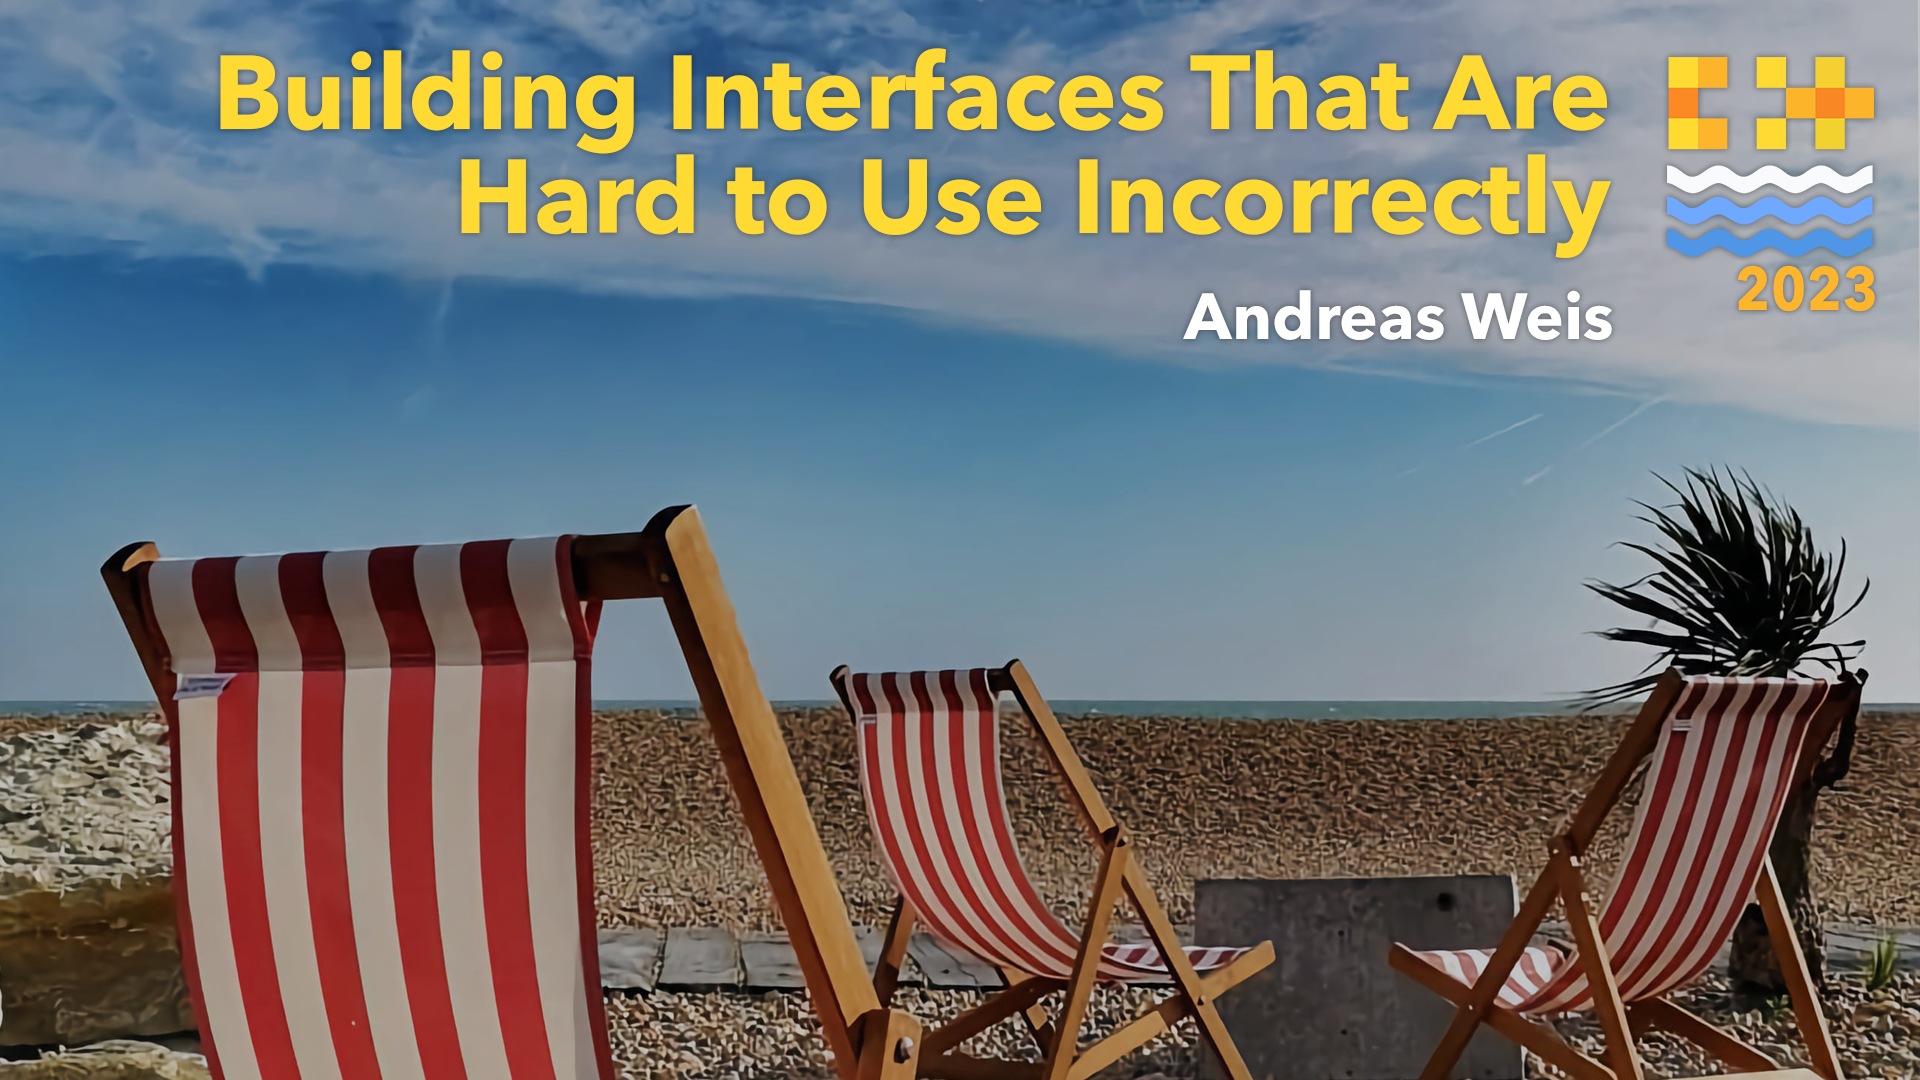
\includegraphics[keepaspectratio,
                                 width=\paperwidth,
                                 height=\paperheight]{ifgfx/title_card_cpponsea.png}
            };
        \end{tikzpicture}
     \end{frame}
}


\frame{\titlepage}

\iftrue %crop
\fi

\begin{frame}[fragile]
  \frametitle{About me - Andreas Weis (he/him)}

  \begin{itemize}
    \setlength\itemsep{1.5em}

    \item \href{https://stackoverflow.com/users/577603/comicsansms}{
\includegraphics[height=.05\textheight]{resources/so-icon.png}} \href{https://github.com/ComicSansMS}{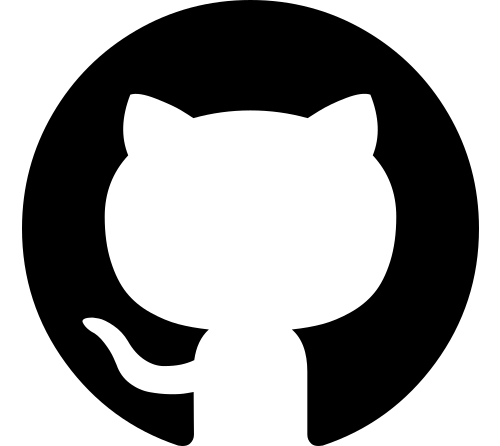
\includegraphics[height=.05\textheight]{resources/github-icon.png}} \includegraphics[height=.05\textheight]{resources/discord-icon.png} ComicSansMS

    %\item \href{https://twitter.com/DerGhulbus/}{
\includegraphics[height=.05\textheight]{resources/twitter-icon.png} @DerGhulbus}

    \item 
\includegraphics[height=.05\textheight]{resources/meetup-icon.png} Co-organizer of the \href{https://www.meetup.com/MUCplusplus/}{Munich C++ User Group}

    \item Currently working as a Vehicle Architect for Woven by Toyota \includegraphics[height=.1\textheight]{resources/woven_toyota_logo.png}

  \end{itemize}
\end{frame}

\begin{frame}
  \frametitle{Motivation}
  
  \begin{center}
  
\includegraphics[height=.9\textheight]{resources/kevlin_97_things.jpg}
  \end{center}

  \note{
  \begin{itemize}
  \item O'Reilly 2010
  \end{itemize}
  }
\end{frame}

\begin{frame}
  \frametitle{Motivation}
  
  \begin{center}
    \begin{tikzpicture}
      \node[opacity=0.1](bgimg) {
\includegraphics[height=.9\textheight]{resources/kevlin_97_things.jpg}};
       \node[align=center,font={\large}] at (bgimg.center) {Item \#55 by Scott Meyers:
       \\
       \textit{Make Interfaces Easy to Use Correctly and Hard to Use Incorrectly}
       };
    \end{tikzpicture}
  \end{center}

  \note{
  \begin{itemize}
  \item O'Reilly 2010
  \end{itemize}
  }
\end{frame}

\begin{frame}

  \frametitle{Motivation}
  
  Good interfaces are:  \vspace{20pt}
  \begin{itemize}
    \item \textbf{Easy to use correctly.}  \vspace{24pt}
  \end{itemize}
  
  \note{
  Item 55 by Scott Meyers: \textit{Make Interfaces Easy to Use Correctly and Hard to Use Incorrectly}
  
  People using a well-designed interface almost always use the interface correctly, because that's the path of least resistance. 
  
  In a GUI, they almost always click on the right icon, button, or menu entry, because it's the obvious and easy thing to do.

  In an API, they almost always pass the correct parameters with the correct values, because that's what's most natural.

  With interfaces that are easy to use correctly, things just work.
  }

\end{frame}

\begin{frame}
  \frametitle{Motivation}
  
  \begin{center}
  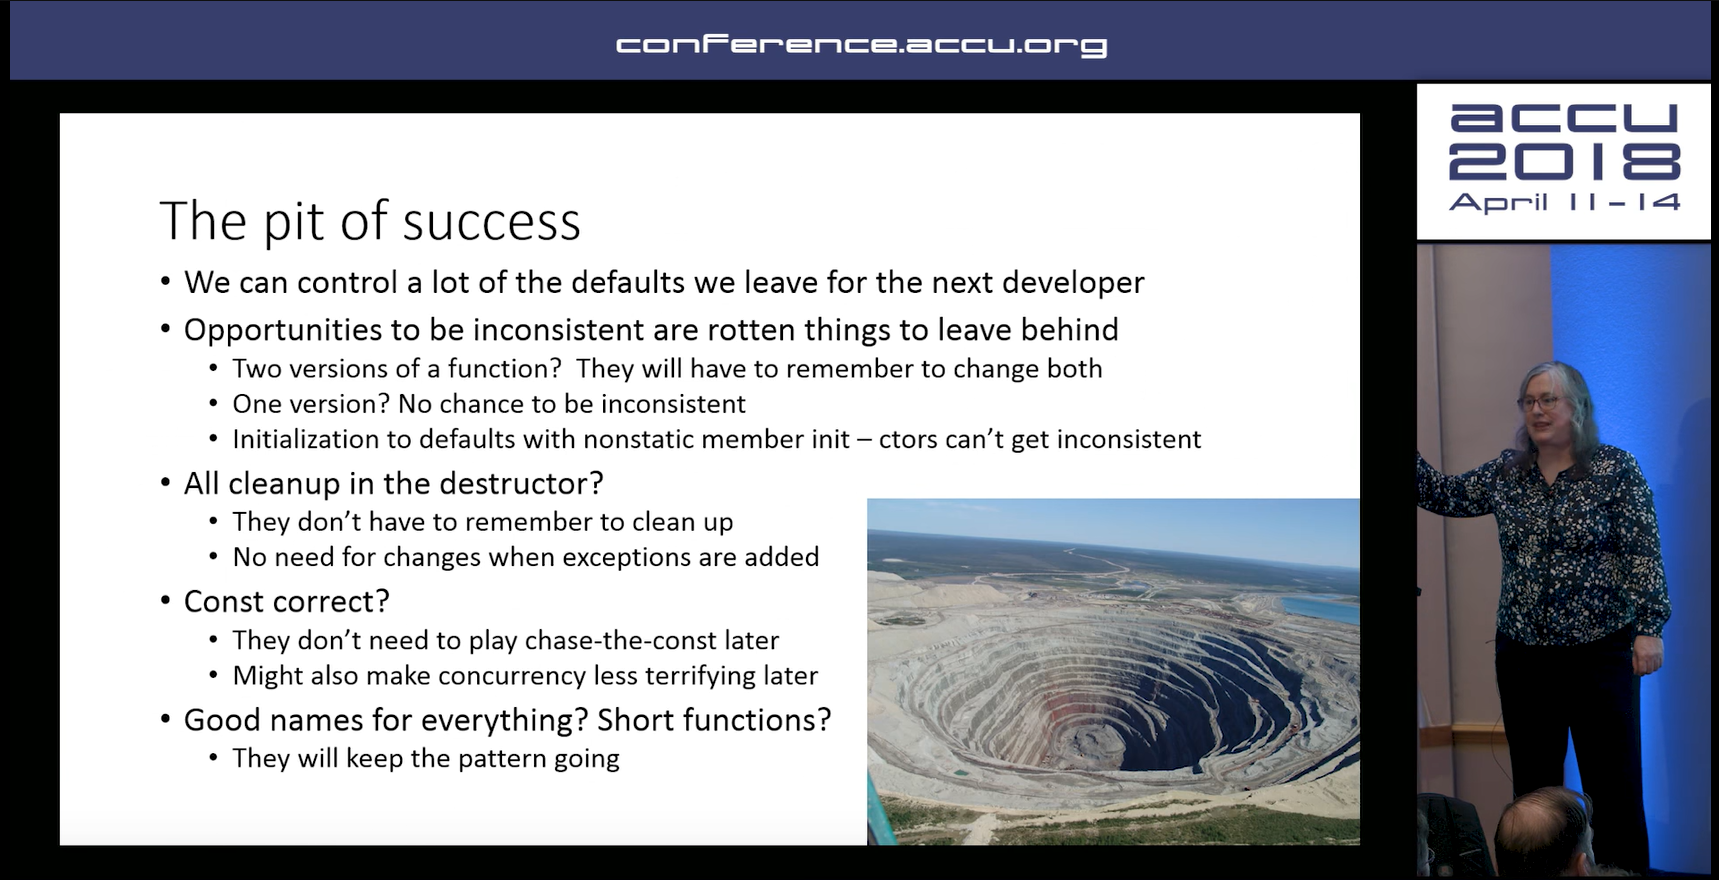
\includegraphics[height=.75\textheight]{resources/kate_pit_of_success.jpg}
  \end{center}

  \href{https://youtu.be/O50qTuM5OT0?t=3460}{Kate Gregory - Simplicity: Not Just for Beginners}

  \note{
  \begin{itemize}
  \item Blog post by Brad Abrams for Microsoft in 2003
  \item Blop post by Jeff Atwood in 2007
  \item Covers the easy to use correctly part
  \item This talk is about \textit{hard to use incorrectly}
  \end{itemize}
  }
\end{frame}

\begin{frame}

  \frametitle{Motivation}
  
  Good interfaces are: \vspace{20pt}
  \begin{itemize}
    \item \textbf{Easy to use correctly.} \vspace{20pt}
    \cpause
    \item \textbf{Hard to use incorrectly.}
  \end{itemize}
  
  \note{
  Item 55 by Scott Meyers: \textit{Make Interfaces Easy to Use Correctly and Hard to Use Incorrectly}
  
  Good interfaces anticipate mistakes people might make and make them difficult — ideally impossible — to commit.

  A GUI might disable or remove commands that make no sense in the current context, for example, or an API might eliminate argument-ordering problems by allowing parameters to be passed in any order.
  }

\end{frame}


\begin{frame}
  \frametitle{Overview}
  \begin{itemize}
    \item Categorization of precondition violations
    \item Leveraging the type system to prevent precondition violations
    \item Techniques for restricting access to data
    \item Techniques for restricting control flow
    \end{itemize}
\end{frame}

\begin{frame}[fragile]
  \frametitle{What is an incorrect use?}
  
  \begin{lstlisting}[style=cpp20]
std::vector<int> v;
v.resize(10);

int i = v[99];
  \end{lstlisting}
\end{frame}

\begin{frame}
  \frametitle{Function Preconditions}
  
  \begin{itemize}
    \item The contract provided of a function can be expressed through \textit{preconditions} and \textit{postconditions}. \cpause
    \item When calling the functions within the defined preconditions, the contract guarantees that the function will establish the postcondtions.  \cpause
    \item When calling the function outside the preconditions, anything can happen. \cpause
  \end{itemize}
  
  \vspace{20pt}
  
  $\Rightarrow$ Violation of preconditions is always an ``incorrect use''.
\end{frame}

\begin{frame}[fragile]
  \frametitle{What is an incorrect use?}
  
  \begin{lstlisting}[style=cpp20]
std::vector<int> v;
v.resize(10);

int i = v.at(99);
  \end{lstlisting}
  
  \vspace{20pt}
  
  \begin{itemize}
    \item Is this incorrect use?
  \end{itemize}
  
  \note{
    \begin{itemize}
      \item New return channel for error
      \item The error return becomes part of the function contract
      \item We provide a wider contract - one that handles more cases
      \item Exceptions try to hide the fact that the contract is widened, but this is not always desirable
    \end{itemize}
  }
\end{frame}

\begin{frame}[fragile]
  \frametitle{What is an incorrect use?}
  
  \begin{lstlisting}[style=cpp20]
float f = std::sqrtf(-1.f);
  \end{lstlisting}
  
  \vspace{20pt}
  
  \begin{itemize}
    \item Is this incorrect use?
  \end{itemize}
  
  \note{
    \begin{itemize}
      \item The error channel is part of the value range of the return type
      \item In this case, a NaN value that taints subsequent operations, propagates similar to an exception
      \item Again will hide the error here but re-surfaces at some other place
    \end{itemize}
  }
\end{frame}

\begin{frame}
  \frametitle{Wide Contracts - Defensive Programming}
  
  \begin{itemize}
    \item Widening a contract reduces the number of preconditions \cpause
    \item Thus a function with a wide contract has seemingly fewer opportunities for incorrect use \cpause
    \item However, the postconditions under the widened contract are usually significantly more complex \cpause
    \item Which again reintroduces new opportunities for incorrect use in other places \cpause
    \item Many preconditions are not detectable \cpause
  \end{itemize}
  
  \vspace{20pt}
  
  $\Rightarrow$ Widening contracts does not prevent ``incorrect use''.
\end{frame}

\begin{frame}[fragile]
  \frametitle{What is an incorrect use?}
  
  \begin{lstlisting}[style=cpp20]
void compute(std::span<std::byte> buffer) {
  // zero out buffer
  std::memset(buffer.data(), buffer.size(), 0);
}
  \end{lstlisting}
  
  \note{
    \begin{itemize}
      \item This is a units error
      \item Confusion between the length of an array and its elements
    \end{itemize}
  }
\end{frame}


\begin{frame}
  \frametitle{Precondition Violations}
  
  \begin{itemize}
    \item Invalid argument
  \end{itemize}
  
  \note{
  \textbf{TIMECHECK}: 0:15
  
  \begin{itemize}
  \item All the examples so far have been invalid argument/domain error
  \item Now we will look at some examples that are not invalid argument errors
  \end{itemize}
  }
\end{frame}

\begin{frame}[fragile]
  \frametitle{What is an incorrect use?}
  
  \begin{lstlisting}[style=cpp20]
  std::fstream fin;
  char buffer[256] = {};
  fin.read(buffer, 256);
  \end{lstlisting}
  
  \note{
    \begin{itemize}
      \item Several issues: Read has a wide contract, but we don't check the error channel
      \item Stream is in wrong state! Should we be able to read from a closed stream?
      \item Form: Must only call read after open().
    \end{itemize}
  }
\end{frame}

\begin{frame}[fragile]
  \frametitle{What is an incorrect use?}
  
  \begin{lstlisting}[style=cpp20]
  std::mutex mtx;
  mtx.lock();
  mtx.lock();
  \end{lstlisting}
  
  \note{
    \begin{itemize}
      \item Locking the mutex twice deadlocks
      \item Form: Must not call lock after lock
    \end{itemize}
  }
\end{frame}

\begin{frame}[fragile]
  \frametitle{What is an incorrect use?}
  
  \begin{lstlisting}[style=cpp20]
  std::vector<int> v = getNumbers();
  auto it_begin = std::ranges::begin(v);
  v.push_back(42);
  int first_element = *it_begin();
  \end{lstlisting}
  
  \note{
    \begin{itemize}
      \item Spooky action at a distance: Changes to the vector invalidate the iterator
      \item Shared mutable state
      \item These are particularly difficult (re: Sean's talk)
    \end{itemize}
  }
\end{frame}

\begin{frame}[fragile]
  \frametitle{What is an incorrect use?}
  
  \begin{lstlisting}[style=cpp20]
  void consumeObject(MyClass&& object);

  MyClass my_object = createObject();
  my_object.doStuff();
  consumeObject(std::move(my_object));
  my_object.doMoreStuff();
  \end{lstlisting}
  
  \note{
    \begin{itemize}
      \item The moved from object is no longer usable
      \item Could be easily prevented by the language, maybe should
      \item Clang Tidy bugprone-use-after-move
    \end{itemize}
  }
\end{frame}



\begin{frame}
  \frametitle{Precondition Violations}
  
  \begin{itemize}
    \item Invalid argument
    \item Invalid context
  \end{itemize}
  
  \cpause
  \vspace{20pt}
  How can we prevent those violations?
  
  \note{
  \begin{itemize}
    \item Sqrt of negative number
    \item Out-of-bounds index
    \item Null pointer argument
  \end{itemize}
  \begin{itemize}
    \item Forget to call init() for two-phase init
    \item Invalidated iterator after resize
    \item Read after file was closed
  \end{itemize}
  }
\end{frame}

\begin{frame}
  \frametitle{Type System to the rescue!}
  
  \cpause
  
  \begin{itemize}
    \item Type system allows us to restrict the set of values assigned to an object \cpause
    \item Type system allows us to restrict the set of operations that can be applied to an object
  \end{itemize}
  
  \note{
  \begin{itemize}
  \item The type system enforces two kinds of restrictions.
  \item These map exactly to the kinds of misuse that we want to address.
  \item We will now look at different techniques for utilizing the type system.
  
  \textbf{TIMECHECK: 0:20}
  \end{itemize}
  }
\end{frame}

\begin{frame}[fragile]
  \frametitle{Opaque Types}
  
  \begin{lstlisting}[style=cpp20]
  void glTexImage2D(
    GLenum target,
    GLint level,
    GLint internalformat,
    GLsizei width,
    GLsizei height,
    GLint border,
    GLenum format,
    GLenum type,
    const void * data);
  \end{lstlisting}
  
  \cpause
  \begin{lstlisting}[style=cpp20]
  glTexImage2D(1, 2, 3, 4, 5, 6, 7, 8, &data);
  \end{lstlisting}
  
  \note{
  \begin{itemize}
  \item Specifying a texture
  \item Lots of parameters for all the different properties of a texture
  \item No protection from incorrect arguments
  \end{itemize}
  }

\end{frame}

\begin{frame}

  \frametitle{Enumerations}

  \begin{itemize}
    \item \texttt{GLenum} is just a typedef for an \texttt{unsigned int}. \cpause
    \item Enumerator values are defined as preprocessor constants. \cpause
    \item Some values even overlap, defining two unrelated enumerators to the same integer value. \cpause
    \item Compiler will never catch an invalid enumerator argument. This is a runtime error at best.
  \end{itemize}

\end{frame}

\begin{frame}[fragile]
  \frametitle{Scoped Enumerators}
  
  \begin{lstlisting}[style=cpp20]
enum class Shape {
  Circle = 1, Square = 2, Triangle = 3
};
enum class Color {
  Red = 1, Green = 2, Blue = 4
};
void setShapeColor(Shape, Color); (*@ \cpause @*)

setShapeColor(Color::Red,
              Shape::Circle);     // does not compile!
Shape s1 = Color::Blue            // does not compile!
Shape s2 = static_cast<Shape>(3); // requires cast
  \end{lstlisting}
\end{frame}

\begin{frame}[fragile]

  \frametitle{Scoped Enumerators as Opaque Typedefs}

  \begin{lstlisting}[style=cpp20]
  enum class Handle : std::uint32_t { Invalid = 0 };
  Handle createResource(); (*@ \cpause @*)
  
  Handle h1 = createResource();
  Handle h2 = Handle::Invalid;  (*@ \cpause @*)
  Handle h3{ 42 };  (*@ \cpause @*)
  Handle h4 = 42;         // does not compile  (*@ \cpause @*)
  enum class OtherHandle : std::uint32_t {};
  OtherHandle h5 = h1;    // does not compile
  \end{lstlisting}
  
  \note{
  Not perfect, but better than plain ints.
  }
\end{frame}


\begin{frame}[fragile]
  \frametitle{Opaque Typedefs}
  
  \begin{lstlisting}[style=cpp20]
template<typename Tag_T>
struct OpaqueHandle { std::uint32_t i; };  (*@ \cpause @*)

struct FileHandleTag {};
using FileHandle = OpaqueHandle<FileHandleTag>;
struct ProcessHandleTag {};
using ProcessHandle = OpaqueHandle<ProcessHandleTag>;  (*@ \cpause @*)

FileHandle openFile(std::filesystem::path);

FileHandle h1 = openFile("important.dat");
ProcessHandle h2 = h1;    // does not compile
  \end{lstlisting}
  
  \note{
  We can get stronger protection if we invest more work.
  Make the \texttt{int} private, restrict construction options...
  }
\end{frame}

\begin{frame}[fragile]
  \frametitle{Opaque Typedefs}
  
  Types defined this way don't support common operations out-of-the-box:
  \begin{itemize}
  \item Compare for equality (\texttt{operator==})
  \item Store in a \texttt{map} (\texttt{operator<})
  \item Store in an \texttt{unordered\_map} (\texttt{std::hash})
  \item Printed to the console (\texttt{operator<<(std::ostream)}, \texttt{std::formatter})
  \item Arithmetic
  \end{itemize}
  
  \cpause
  
  Libraries like \href{https://github.com/rollbear/strong_type}{Björn Fahller's \texttt{strong\_type}} provide customizable opaque types.
  
  Arithmetic is supported by units libraries like \href{https://github.com/mpusz/units}{Mateusz Pusz's mp-units}.
\end{frame}

\begin{frame}[fragile]
  \frametitle{Structuring arguments}
  
  \begin{lstlisting}[style=cpp20]
void* memset(void* buffer, int fill_char,
             size_t buffer_size);
  
memset(buffer, 10, 20);
  \end{lstlisting}

  \cpause

  \vspace{10pt}
  Compare with:

  \begin{lstlisting}[style=cpp20]
void* my_memset(std::span<std::byte> span, int fill_char);
  
my_memset(std::span(buffer, 20), 10);
  \end{lstlisting}
  
  \note{
  \textbf{TIMECHECK}: 0:30
  
  Second version is harder to get wrong and more expressive on caller side
  }
\end{frame}


\begin{frame}[fragile]
  \frametitle{Structuring arguments}

  \begin{lstlisting}[style=cpp20]
struct MemsetArgs {
  void* buffer;
  size_t size;
  int fill_char;
};
void* my_memset(MemsetArgs const& args);  (*@ \cpause @*)
  
my_memset({ .buffer = b, .size = 20, .fill_char = 10 });
  \end{lstlisting}
  
  \note{
  Designated initializers with C++20 is the game changer here
  }
\end{frame}

\begin{frame}[fragile]
  \frametitle{Structuring arguments}
  
  \begin{lstlisting}[style=cpp20]
Rectangle r1{10, 20, 30, 40};

Rectangle r2{Point{ .x = 10, .y = 20 },
             Point{ .x = 30, .y = 40 }};

Rectangle r3{Point{ .x = 10, .y = 20 },
             Extents{ .width = 30, .height = 40 }};
  \end{lstlisting}
\end{frame}


\begin{frame}[fragile]
  \frametitle{Structured Data Access}
  
  \begin{lstlisting}[style=cpp20]
using Shape = std::variant<Rectangle, Circle, Triangle>;

Shape s = getShape(); (*@ \cpause @*)

if (std::holds_alternative<Circle>(s)) {
  float r = std::get<Circle>(s).getRadius();
}
  \end{lstlisting}
  
  \note{
  Easy to mess up:
  \begin{itemize}
    \item I forget to handle one case
    \item breaks silently when adding new shapes.
  \end{itemize}
  }
\end{frame}

\begin{frame}[fragile]
  \frametitle{Structured Data Access}
  
  \begin{lstlisting}[style=cpp20]
float getArea(Rectangle const& r);
float getArea(Circle const& c);
float getArea(Triangle const& t);

Shape my_shape = getShape();
float const area = std::visit(
  [](auto const& s) { return getArea(s); },
  my_shape);
  \end{lstlisting}
\end{frame}

\begin{frame}[fragile]
  \frametitle{Structured Data Access}
  
  \begin{lstlisting}[style=cpp20]
template<class... Ts>
struct overloaded : Ts... { using Ts::operator()...; };

Shape my_shape = getShape();
std::visit(overloaded{
  [](Rectangle const& r) { /* ... */ }
  [](Circle const& c) { /* ... */ }
  [](Triangle const& t) { /* ... */ }
});
  \end{lstlisting}
\end{frame}

\iffalse
\begin{frame}[fragile]
  \frametitle{Data Types with special properties}

Consider these alternatives:

  \begin{lstlisting}[style=cpp20]
// \pre Widget must not be nullptr
void processWidget(Widget* w);

void processWidget(Widget& w);

void processWidget(gsl::not_null<Widget*> w);
  \end{lstlisting}
\end{frame}

\begin{frame}[fragile]
  \frametitle{Data Types with special properties}

Consider these alternatives:
  \begin{lstlisting}[style=cpp20]
// \pre str must be a null-terminated string
void processString(char const* str);

void processString(std::string_view str);

void processString(gsl::czstring str);
  \end{lstlisting}
\end{frame}
\fi

\begin{frame}[fragile]
  \frametitle{Limited Friendship}
  
  \begin{lstlisting}[style=cpp20]
class Database {
  Internals m_privateState;
public:
  Data retrieveData(Handle h);
private:
  Data retrievePrivilegedData(Handle h);
};

class Client;
class PrivilegedClient;
  \end{lstlisting}
  
  \note{
  \textbf{TIMECHECK}: 0:35
  }
\end{frame}

\begin{frame}[fragile]
  \frametitle{Limited Friendship - Passkey Idiom}
  
  \begin{lstlisting}[style=cpp20]
struct AccessToken {
private:
    AccessToken() = default;
    friend class PrivilegedClient;
};

class Database {
  Internals m_privateState;
public:
  Data retrieveData(Handle h);
  Data retrievePrivilegedData(Handle h, AccesToken t);
};
  \end{lstlisting}
  
  See Arne's blog: \href{https://arne-mertz.de/2016/10/passkey-idiom/}{Passkey Idiom: More Useful Empty Classes}
\end{frame}

\begin{frame}[fragile]
  \frametitle{Declarative Interface}
  
  \begin{lstlisting}[language={C}]
in vec3 Position;
in vec3 Normal;
in vec2 TexCoord;
  \end{lstlisting}
  
  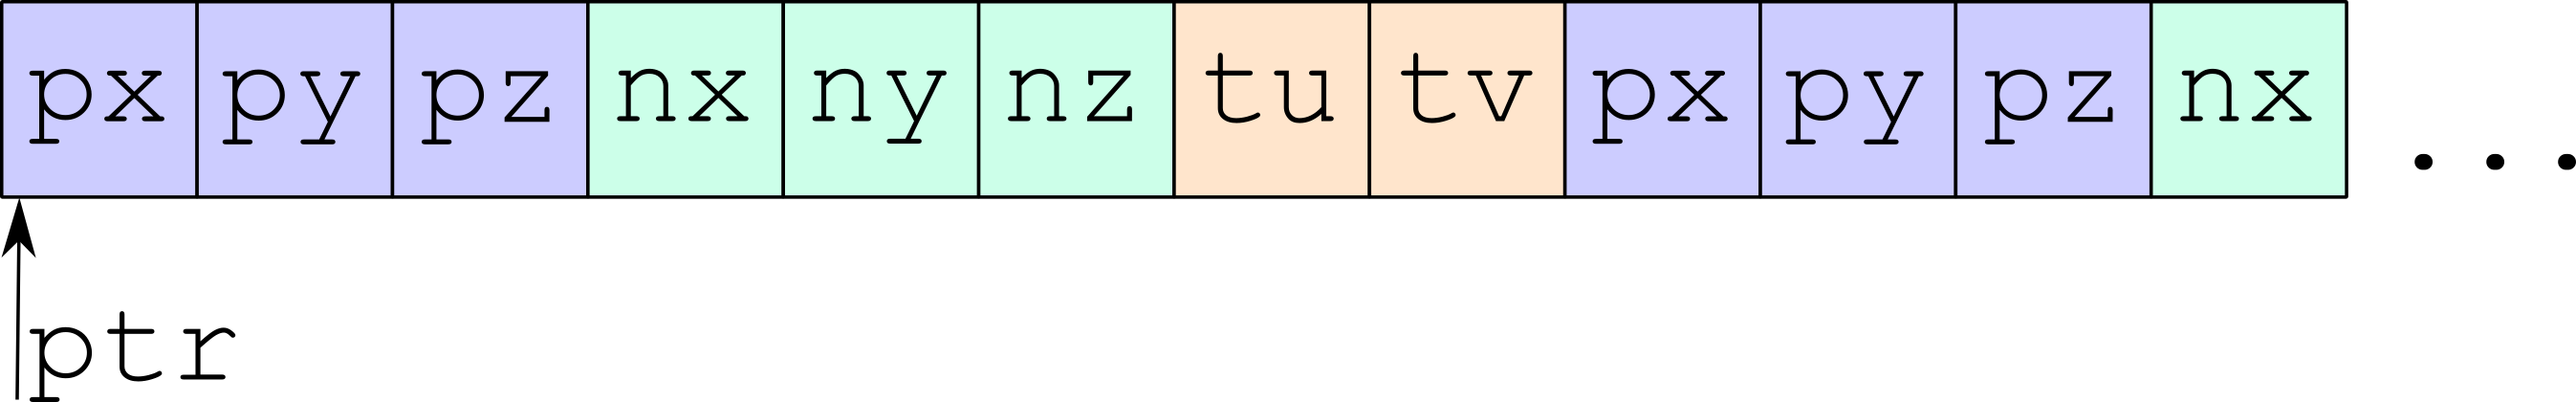
\includegraphics[width=0.9\textwidth]{ifgfx/vertex_buffer_0.png}
  
  \begin{lstlisting}[style=cpp20]
glBufferData(GL_ARRAY_BUFFER, size, ptr, ...);
glVertexAttribPointer(index_pos, 3, GL_FLOAT,
                      stride, offset_pos);
// ...
  \end{lstlisting}
  
  \note{
  \begin{itemize}
  \item Geometry data starts its life as structured data in C++.
  \item Data gets memcopied into a single buffer that is transferred to the GPU.
  \item Location of the individual vertex components inside this buffer are configured through a series of \texttt{glVertexAttribPointer} calls.
  \end{itemize}
  }
\end{frame}

\iffalse
\begin{frame}[fragile]
  \frametitle{Declarative Interface}
  
  \begin{lstlisting}[style=cpp20]
struct Vertex {
  Vec3 position;
  Vec3 normal;
  Vec2 textureCoordinate;
};
std::vector<Vertex> vertex_buffer;
  \end{lstlisting}
  
  \begin{itemize}
  \item Geometry data starts its life as structured data in C++.
  \item Data gets memcopied into a single buffer that is transferred to the GPU.
  \item Location of the individual vertex components inside this buffer are configured through a series of \texttt{glVertexAttribPointer} calls.
  \end{itemize}
\end{frame}
\fi

\begin{frame}[fragile]
  \frametitle{Declarative Interface}
  \begin{lstlisting}[style=cpp20]
using MyFormat = VertexFormat<
  Component::Position3f,
  Component::Normal3f,
  Component::TexCoord2f
>;

shader.bind<MyFormat, Component::Position3f>("Position");
shader.bind<MyFormat, Component::Normal3f>("Normal");
shader.bind<MyFormat, Component::TexCoord2f>("TexCoord");
  \end{lstlisting}
\end{frame}

\begin{frame}
  \frametitle{Declarative Interface}
  
  \begin{itemize}
  \item Specify the \textit{what} instead of the \textit{how}
  \item Restrict the parameter space to a set of predefined sensible values
  \item Leave just enough room for customization for what is sensible for the domain
  \item Deduce the tricky configuration parameters from the declarative description
  \end{itemize}
  
  Higher-level interface is potentially more restrictive than the lower-level one. Consider leaving an escape hatch for exotic use cases.
\end{frame}

\begin{frame}[fragile]
  \frametitle{Modeling State Through Types}
  \cpause
  \begin{lstlisting}[style=cpp20]
class Widget {
public:
  // Constructs an uninitialized widget.
  Widget();
  //! Initializes the widget.
  //! \pre Widget must not have been initialized.
  void init();
  //! \pre Widget must have been initialized.
  void doStuff();
};
  \end{lstlisting}
  
  \note{
  \textbf{TIMECHECK}: 0:40
  }
\end{frame}

\begin{frame}[fragile]
  \frametitle{Two-Phase Initialization}

  \begin{lstlisting}[style=cpp20]
class Widget {
  Widget();
  void init();
public:
  void doStuff();
  friend Widget createWidget();
};

Widget createWidget() {
  Widget w;
  w.init();
  return w;
}
  \end{lstlisting}
  
  \note{
  First attempt: wrap the initialization
  }
\end{frame}

\begin{frame}[fragile]
  \frametitle{Two-Phase Initialization}

  \begin{lstlisting}[style=cpp20]
class UninitializedWidget {
public:
  UninitializedWidget();
}; (*@ \cpause @*)
class Widget {
private:
  Widget();
public:
  void doStuff();
}; (*@ \cpause @*)

Widget initializeWidget(UninitializedWidget&& w);
  \end{lstlisting}
  
  \note{
  \begin{itemize}
  \item Converting the type by consuming the source object - functional update 
  \item Functional update changes the value
  \item If the operation depends on the value, it has to change the type as well
  \end{itemize}
  }
\end{frame}

\iffalse
\begin{frame}[fragile]
  \frametitle{Error Handling Paradigms}
  
Consider these alternatives:
  \begin{lstlisting}[style=cpp20]
// Returns 0 on success, error code on failure.
Result_T retrieveFrob(Frob* out_frob);

// Sets errno in case of failure
Frob retrieveFrob();

// Throws in case of failure
Frob retrieveFrob();
  \end{lstlisting}
\end{frame}

\begin{frame}[fragile]
  \frametitle{C++23 \texttt{std::expected}}
  
  \begin{lstlisting}[style=cpp20]
std::expected<Frob, Error_T> retrieveFrob() {
  if (!frobState.isGood()) {
    return std::unexpected(Error_T::BadFrob);
  }
  return frobState;
}
  \end{lstlisting}
  \cpause
  \begin{lstlisting}[style=cpp20]
std::expected<Frob, Error_T> f = retrieveFrob();
if (!f) {
  // handle error
} else {
  f->doStuff();
}
  \end{lstlisting}
\end{frame}

\begin{frame}[fragile]
  \frametitle{C++23 \texttt{std::expected}}
  
  \begin{lstlisting}[style=cpp20]
std::expected<Frob, Error_T> retrieveFrob() {
  if (!frobState.isGood()) {
    return std::unexpected(Error_T::BadFrob);
  }
  return frobState;
}

f.value_or(defaultFrob).doStuff();




.
  \end{lstlisting}
\end{frame}
\fi

\begin{frame}[fragile]
  \frametitle{Execution Tokens}
  
  \begin{itemize}
  \item Restrict the circumstances under which a function may be executed.
  \item Only allow the execution of a function in specific contexts, e.g. within a transaction, when a lock is held, when a resource is available, etc.
  \item Scope in which the relevant context is active is reflected by the program structure.
  \end{itemize}
\end{frame}

\begin{frame}[fragile]
  \frametitle{Execution Tokens}
  
  \begin{lstlisting}[style=cpp20]
class ExecutionToken {
private:
  ExecutionToken();
}; (*@ \cpause @*)
class Provider {
public:
  ExecutionToken establishContext();
}; (*@ \cpause @*)

class Widget {
public:
  void process(ExecutionToken&& token);
};
  \end{lstlisting}
  
  \note{
  \begin{itemize}
    \item Unlike the functional update, we don't have to move the full object state around
    \item Models one-off events: Establishing the context allows us to execute one operation
    \item C++ move semantics allow us to retain a consumed execution token (e.g. in a member variable). Again, external tools can help prevent this.
  \end{itemize}
  }
\end{frame}

\iffalse
\begin{frame}
  \frametitle{Execution Tokens}
  \begin{itemize}
    \item Models one-off events: Establishing the context allows us to execute one operation
    \item C++ move semantics allow us to retain a consumed execution token (e.g. in a member variable). Again, external tools can help prevent this.
  \end{itemize}
\end{frame}
\fi

\begin{frame}[fragile]
  \frametitle{Scoped Execution Contexts}
  
  \begin{lstlisting}[style=cpp20]
  vkBeginCommandBuffer(cmd_buffer, &args);
    vkCmdCopyImage(cmd_buffer, ...);
    vkCmdBeginRenderPass(cmd_buffer, ...);
      vkCmdBindVertexBuffers(cmd_buffer, ...);
      vkCmdDraw(cmd_buffer, ...);
    vkCmdEndRenderPass(cmd_buffer, ...);
  vkEndCommandBuffer(cmd_buffer);
  \end{lstlisting}
  
  \note{
  \textbf{TIMECHECK}: 0:50
  }
\end{frame}

\begin{frame}[fragile]
  \frametitle{Scoped Execution Contexts}
  
  \begin{lstlisting}[style=cpp20]
class CommandRecorder {
  void cmdCopyImage(...);
  RenderPassRecorder beginRenderPass(...);
};

class RenderPassRecorder {
  void cmdBindVertexBuffers(...);
  void cmdDraw(...);
};

class CommandBuffer {
  CommandRecorder begin();
};
  \end{lstlisting}
\end{frame}

\begin{frame}[fragile]
  \frametitle{Scoped Execution Contexts}
  
  \begin{lstlisting}[style=cpp20]
CommandRecorder beginCommandBuffer(CommandBuffer&&);
CommandBuffer endCommandBuffer(CommandRecorder&&);
RenderPassRecorder beginRenderPass(CommandRecorder&&);
CommandRecorder endRenderPass(RenderPassRecorder&&);
  \end{lstlisting}
  
  \begin{lstlisting}[style=cpp20]
CommandBuffer cmd_buffer = ...;
auto cmd_recorder = beginCommandBuffer(std::move(cmd_buffer), ...);
cmd_recorder.cmdCopyImage(...);
cmd_buffer = endCommandBuffer(std::move(cmd_recorder));
  \end{lstlisting}
\end{frame}


\begin{frame}[fragile]
  \frametitle{Complex State Machines}
  
  \begin{center}
  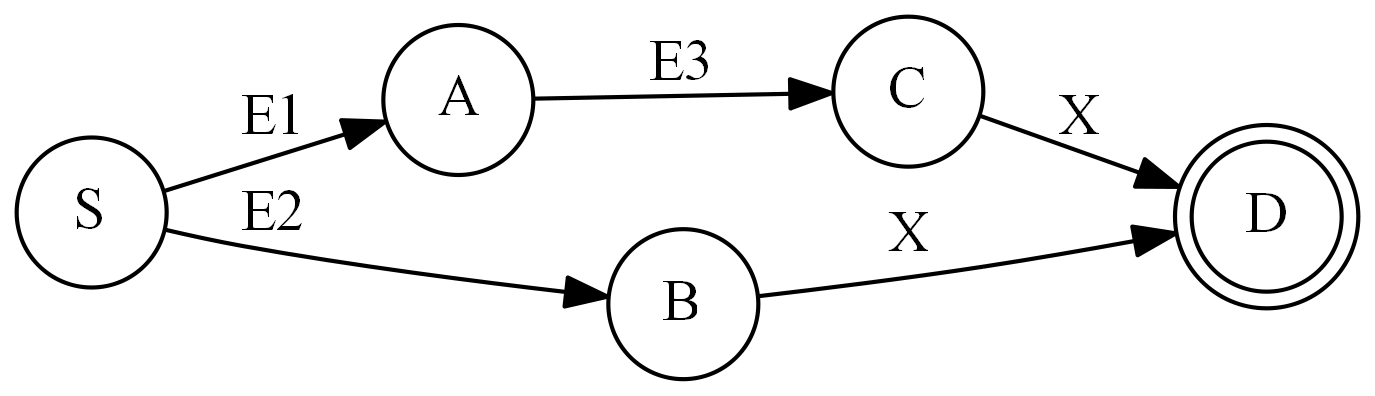
\includegraphics[width=.9\textwidth]{ifgfx/state_machine.png}
  \end{center}
\end{frame}

\begin{frame}[fragile]
  \frametitle{Complex State Machines}
  
  \begin{center}
  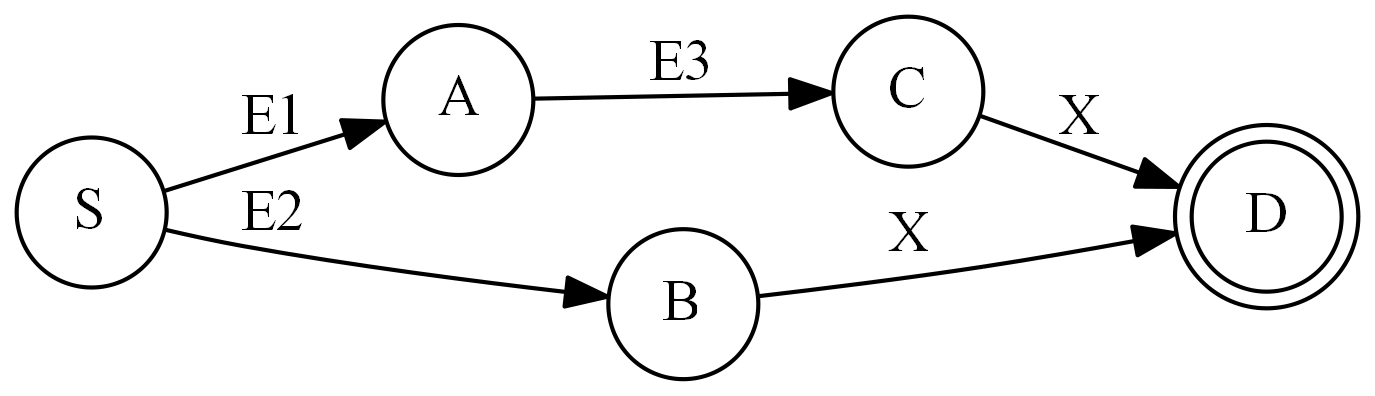
\includegraphics[width=.4\textwidth]{ifgfx/state_machine.png}
  \end{center}
  
  \begin{lstlisting}[style=cpp20]
namespace State {
  class S;
  class A;
  // ...
}
namespace Events {
  class E1;
  // ...
}
  \end{lstlisting}
\end{frame}

\begin{frame}[fragile]
  \frametitle{Complex State Machines}
  
  \begin{lstlisting}[style=cpp20]
State::S initial_state;
State::A state_a =
  transition(std::move(initial_state), Events::E1{});
State::B state_c =
  transition(std::move(state_a), Events::E3{});
  \end{lstlisting}
\end{frame}

\begin{frame}[fragile]
  \frametitle{Complex State Machines}
  
  \begin{itemize}
  \item Gives full control over the possible state transitions and available interfaces for each state.
  \item Leaves behind a dead state object with each transition.
  \item No uniform storage for states - type erased storage again loses all of the compile-time control.
  \end{itemize}
\end{frame}

\begin{frame}[fragile]
  \frametitle{The GoF State Pattern}
  
  \begin{lstlisting}[style=cpp20]
struct State {
  virtual ~State() = default;
  virtual void doStuff() = 0;
};
struct StateA : public State { /* ... */ };
struct StateB : public State { /* ... */ }; (*@ \cpause @*)

class Context {
  std::unique_ptr<State> m_state;
public:
  void doStuff() { m_state->doStuff(); }
  void setState(StateDesc new_state);
};
  \end{lstlisting}
\end{frame}

\iffalse %!!!!!!!!!!!!!!!!!

\fi %!!!!!!!!!!!!!!!!!

\begin{frame}
  \frametitle{Conclusion}
  
  \begin{itemize}
  \item Harden interfaces by making it impossible to violate preconditions without widening the contract.
  \item Two fundamental classes of preconditions: Restrictions on arguments and restrictions on context.
  \item A variety of techniques exist to move precondition checks to compile-time.
  \item Difficult trade-offs between correctness and implementation effort and usability.
  \end{itemize}
  
  \note{
  \textbf{TIMECHECK}: 0:55
  }
\end{frame}

\begin{frame}
  \frametitle{Thanks for your attention.}

  \href{https://stackoverflow.com/users/577603/comicsansms}{
\includegraphics[height=.05\textheight]{resources/so-icon.png}}
  \href{https://github.com/ComicSansMS}{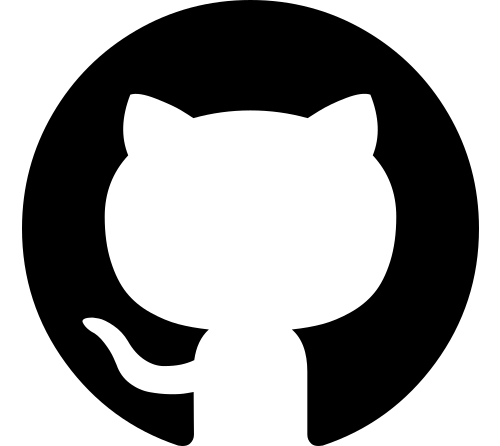
\includegraphics[height=.05\textheight]{resources/github-icon.png}}
  \includegraphics[height=.05\textheight]{resources/discord-icon.png} ComicSansMS
  %\includegraphics[height=.05\textheight]{resources/discord-icon.png} ComicSansMS /
  %\href{https://twitter.com/DerGhulbus/}{
\includegraphics[height=.05\textheight]{resources/twitter-icon.png} @DerGhulbus}

\end{frame}


\end{document}
